%timeseries are every where (with forecasting)
%Modeling time sreeis
%seasonality 
%-decomping a time series
%-forecast using decomposed 
%important of integerating 

Time series are encountered in many applications, including financial (e.g., stock price~\cite{stock}) and scientific database (e.g.,
sensor data for weather information~\cite{arimaEng} or other environmental data).
Due to the importance and wide spread of time series,  forecasting time series is essential for  many applications. For example, in stock trading a forecast method based on  neural networks  has been proposed~\cite{stock}.
In energy domain, several forecasting methods including exponential smoothing \cite{} and ARIMA~\cite{tBOX76a} have been used.
Even in foreign politics relationship, a forecast models exist~\cite{iran}.

%query time series
For time series, it is  critical to integrate past and future data for two folds: first, to forecast future values in a time series, a forecast method  accesses past values.   Secondly, as the time passes, the transition of forecasted values to historic values should be seamlessly supported. Furthermore, the forecasted value  may be used until the actual value becomes available.   Consider the following query from  energy domain: the power grid operator investigates when the power consumption exceeded (or will exceed) a certain limit of the network  over the previous and upcoming weeks. Like 
 (e.g.,\cite{AG99}, \cite{BlinkDB} and \cite{KML10}), we use threshold and confidence to speedup the query execution. 
Consider for our example, an approximate answer with 1\% error  and 95\% confidence is adequate.
\begin{verbatim}
SELECT time, load
FROM   Power_consumption
WHERE current_load>limit AND
time in INTERVAL time in [NOW-WEEK , NOW + WEEK]      
ERROR WITHIN 10% AT CONFIDENCE 95% ERROR  1%
CONFIDENCE  95%
\end{verbatim}
 A naive approach to answer this query would scan the data points over the previous week, optimize parameters for a forecast method, and predict the time series for the next week. Finally, the query discards values that are lower than the specified threshold. Our proposed system performs this more intelligently, as will be explain next. 


Several approaches have been proposed to approximate a time series including Piecewise Aggregate Approximation (PAA), Adaptive Piecewise Constant Approximation (APCA),  Symbolic Aggregate approXimation (SAX). These approaches focus on similarity and querying time series by content.
Traditionally, a time series  can be decomposed into a trend component, a seasonal component, and a local (i.e., stationary) component~\cite{Decompose}. 

%Several techniques have been proposed to model  time series 
 
 %seasonality and model time series modeling
 % decomposing time series and use it to
Typically, a real-world time series  exhibit at least one  seasonal behaviors. For instance, household power consumption rises in winter and during the day and falls in the summer and at night.
Therefore, statistical  forecasting methods (e.g., ARIMA~\cite{tBOX76a}) use these components  to accurately compute forecast values. 	






Ignoring the time series seasonality  results in (1) increasing the number of models needed to approximate the time series [past](2) []future]. 




%remedy (it to model each compoment indedently)


   
 %For our purpose, we abstract a forecast method as a function of forecast parameters and states (i.e., past values) and outputs future values. We use this decomposition to represent the time series over the past and the future.
 
 %intergrating time series and forecast
 

%Modeling has been extensively used in different applications including forecasting, estimating, approximating, neuroscience, and rendering graphics for computer games.
%Because forecast methods could not be used to store historical data, we  model historical data separately.
%These seasonal components have periods of 10 and 5 cycles, respectively.
A time series  can be decomposed into a trend component, a seasonal component, and a local (i.e., stationary) component~\cite{Decompose}. 
%example
Throughout the paper, we use our motivating example shown in Figure~\ref{fig:example}. 
Figure~\ref{fig:example}a gives 50 values which is based on real-world household power consumption in UK.  This time series can be decomposed to three components: two seasonal with period length of 5 and 10  and one trend components, the decomposed components are  shown in Figure~\ref{fig:example}b. 
By storing the complements instead of the original timeseries,  we can greatly reduce the storage requirements. In this toy example, instead of storing  50 values of the original time series, we need only to store 19 values to exactly represent the time series (i.e., with 0\% error and 100\% confidence). This can be acoomplished by storing  four trends values and  10 and five seasonality periods. This corresponds to a compression ratio of 42\%. Moreover, we can easily forecast the time series by exaggerating the decomposed components.
\begin{figure*}[th]
\center
\subfigure{
\includegraphics[width=2.0in]{figs/example.eps}}
\subfigure{
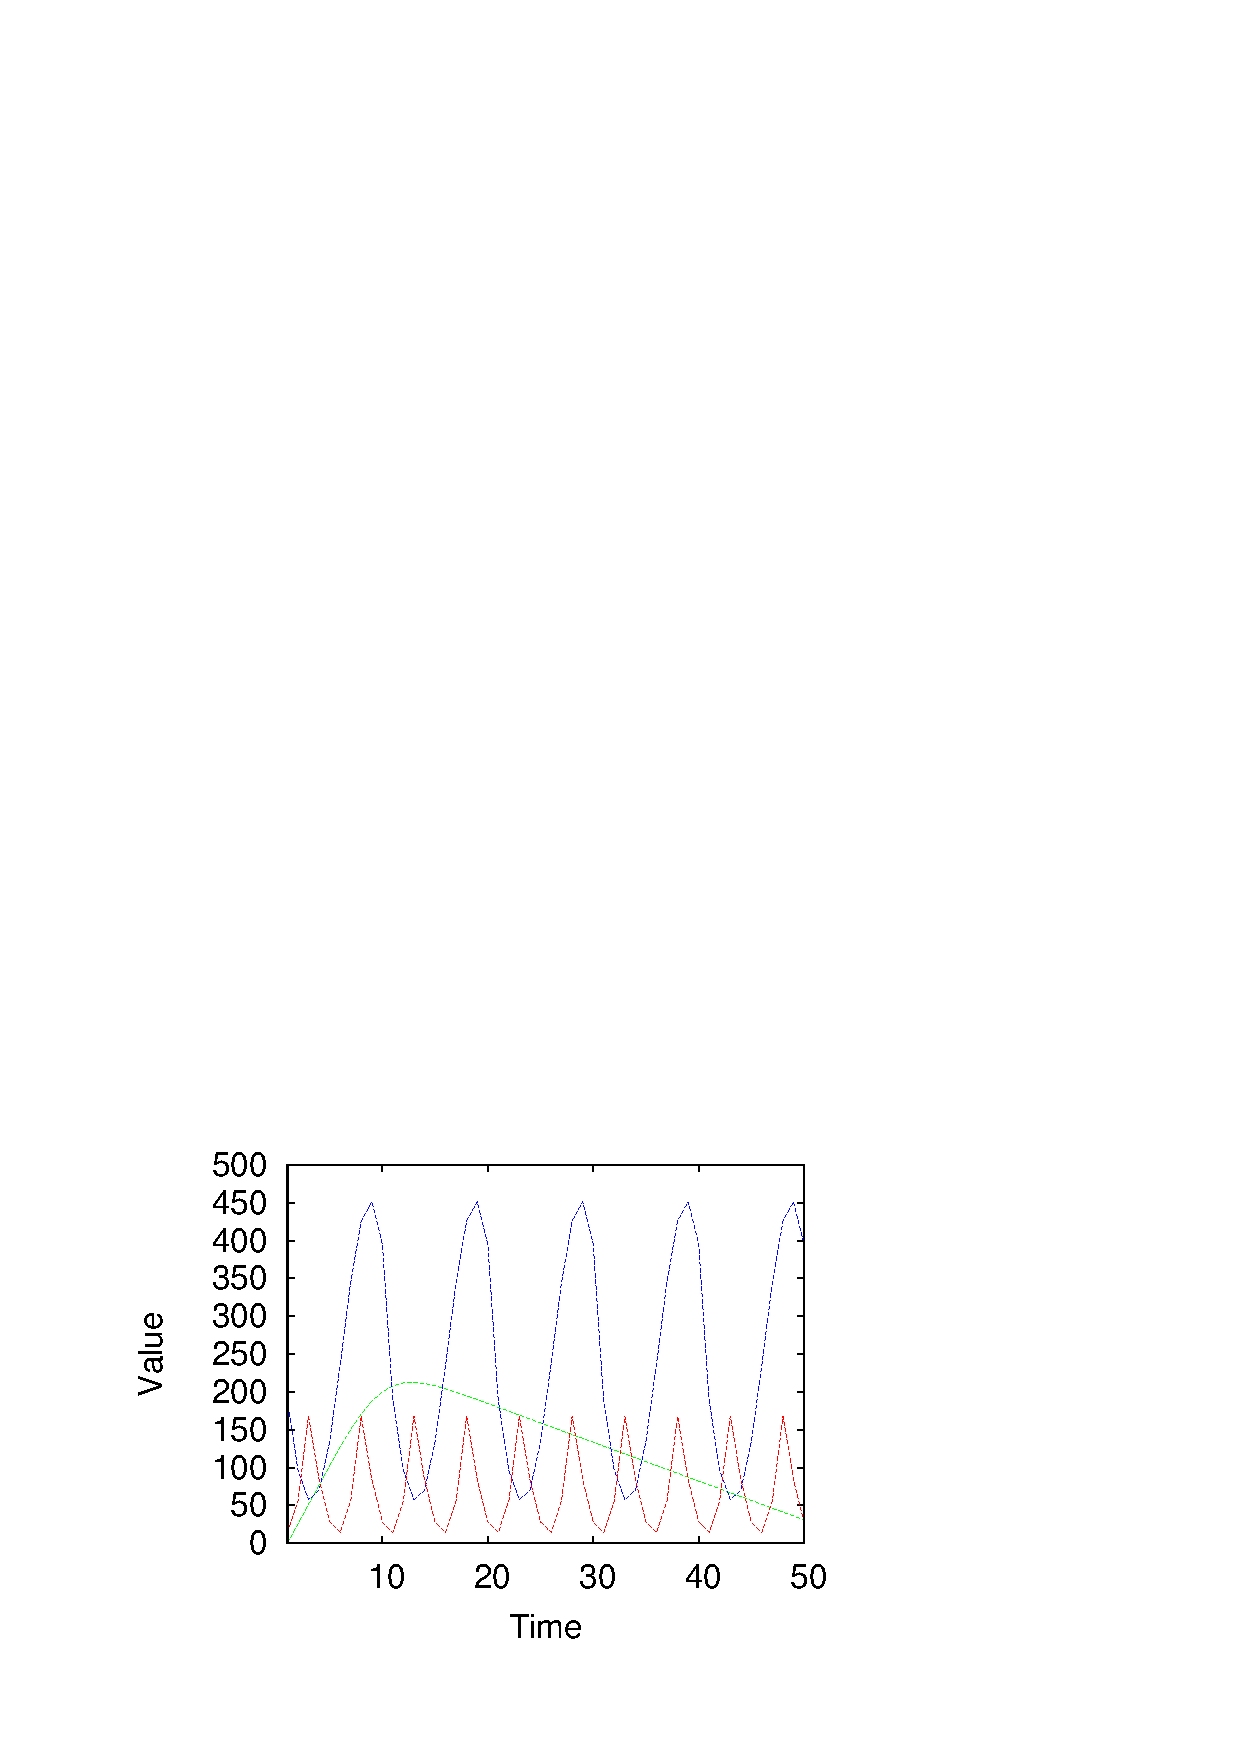
\includegraphics[width=2.0in]{figs/example_compoments.pdf}}
\caption{Motivating Example}
\label{fig:example}
\end{figure*} 

% As approximate answers can be computed order-of-magnitude faster than their counterpart exact queries. Therefore, our system support computing approximate queries within error guarantees over future and historic data.
%our system
To this end, we introduce a  TimeTravel, an efficient DBMS system for seamless integration  of past and future time series values, supporting two types of queries:
(a)~approximate queries on past and future within user-specified error bounds (i.e., absolute error and confidence), and (b)~exact historic queries.
We can support point, range, aggregate and join queries.
Unlike, previous approaches, we utilize trend and seasonality components to build models over the underlying time series to support . Ignoring seasonality components results in low compression ratio as we will discuss later.  Here, past and future data is treated similarly, allowing seamless integrated querying. The main difference of future data compared to past is that the (estimated) error is typically higher.
To organize these models and efficiently support queries with various error guarantees, we introduce a novel index structure, denoted as {\em \LN}.  The upper levels in the index are more ``coarse-grained'', representing 
the underlying time series with a higher error and a lower confidence and fewer model segments compared to the lower levels which are more accurate. Please note that confidence while building models to reduce the effect of  {\it outliers} on the quality of models.

For approximate historical queries (e.g., last week in our motivating example), we use the highest-level models to calculate an approximate answer. If the  answer violates the user requirements on error and confidence, we consult relevant models at lower levels.  We continue traversing the hierarchical model index until either the error guarantee given by user is met or the underlying time series is accessed.
In addition, TimeTravel efficiently answers exact queries by utilizing the index  to find the relevant portions in the time series. For example, considering MIN aggregation queries, we only access the portion of the time series where the minimum value might exist. 
For future queries (e.g., next week in our motivating example), we use the model index to retrieve forecast states which is supplemented to  statistical forecast methods.
We meet the user required error guarantees on future data by (a)~controlling the error and confidence of the  retrieved forecast states and (b)~optimizing the forecast method parameters. 

To build the hierarchical model index, the user specifies hints for: (1)~seasonality periods, (2)~error guarantees levels, and (3)~the statistical forecast method (e.g., ARIMA).  
We recursively divide the time series into non-overlapping intervals and build a model on each interval until all error requirements are satisfied. 
Over time, {\it new} values are added to the time series, and we incrementally update the parameters for the forecast method and add  models to the hierarchical model index.

In the rest of this paper, first we formalize the problem statements in Section~\ref{sec:form}.   Section~\ref{sec:overview} provides an overview of the our proposed system. Section~\ref{sec:details} describes building the hierarchical model index, and  compression Section~\ref{sec:query} gives the details of query optimization and processing for approximate and exact queries.  The  related work is presented in Section~\ref{sec:related}. Section~\ref{sec:experiments} gives  our experimental analysis for our proposed system   using  both real-world time series data and synthetic data.

%\section{Running Example}
%\begin{figure*}[th]

%\center
%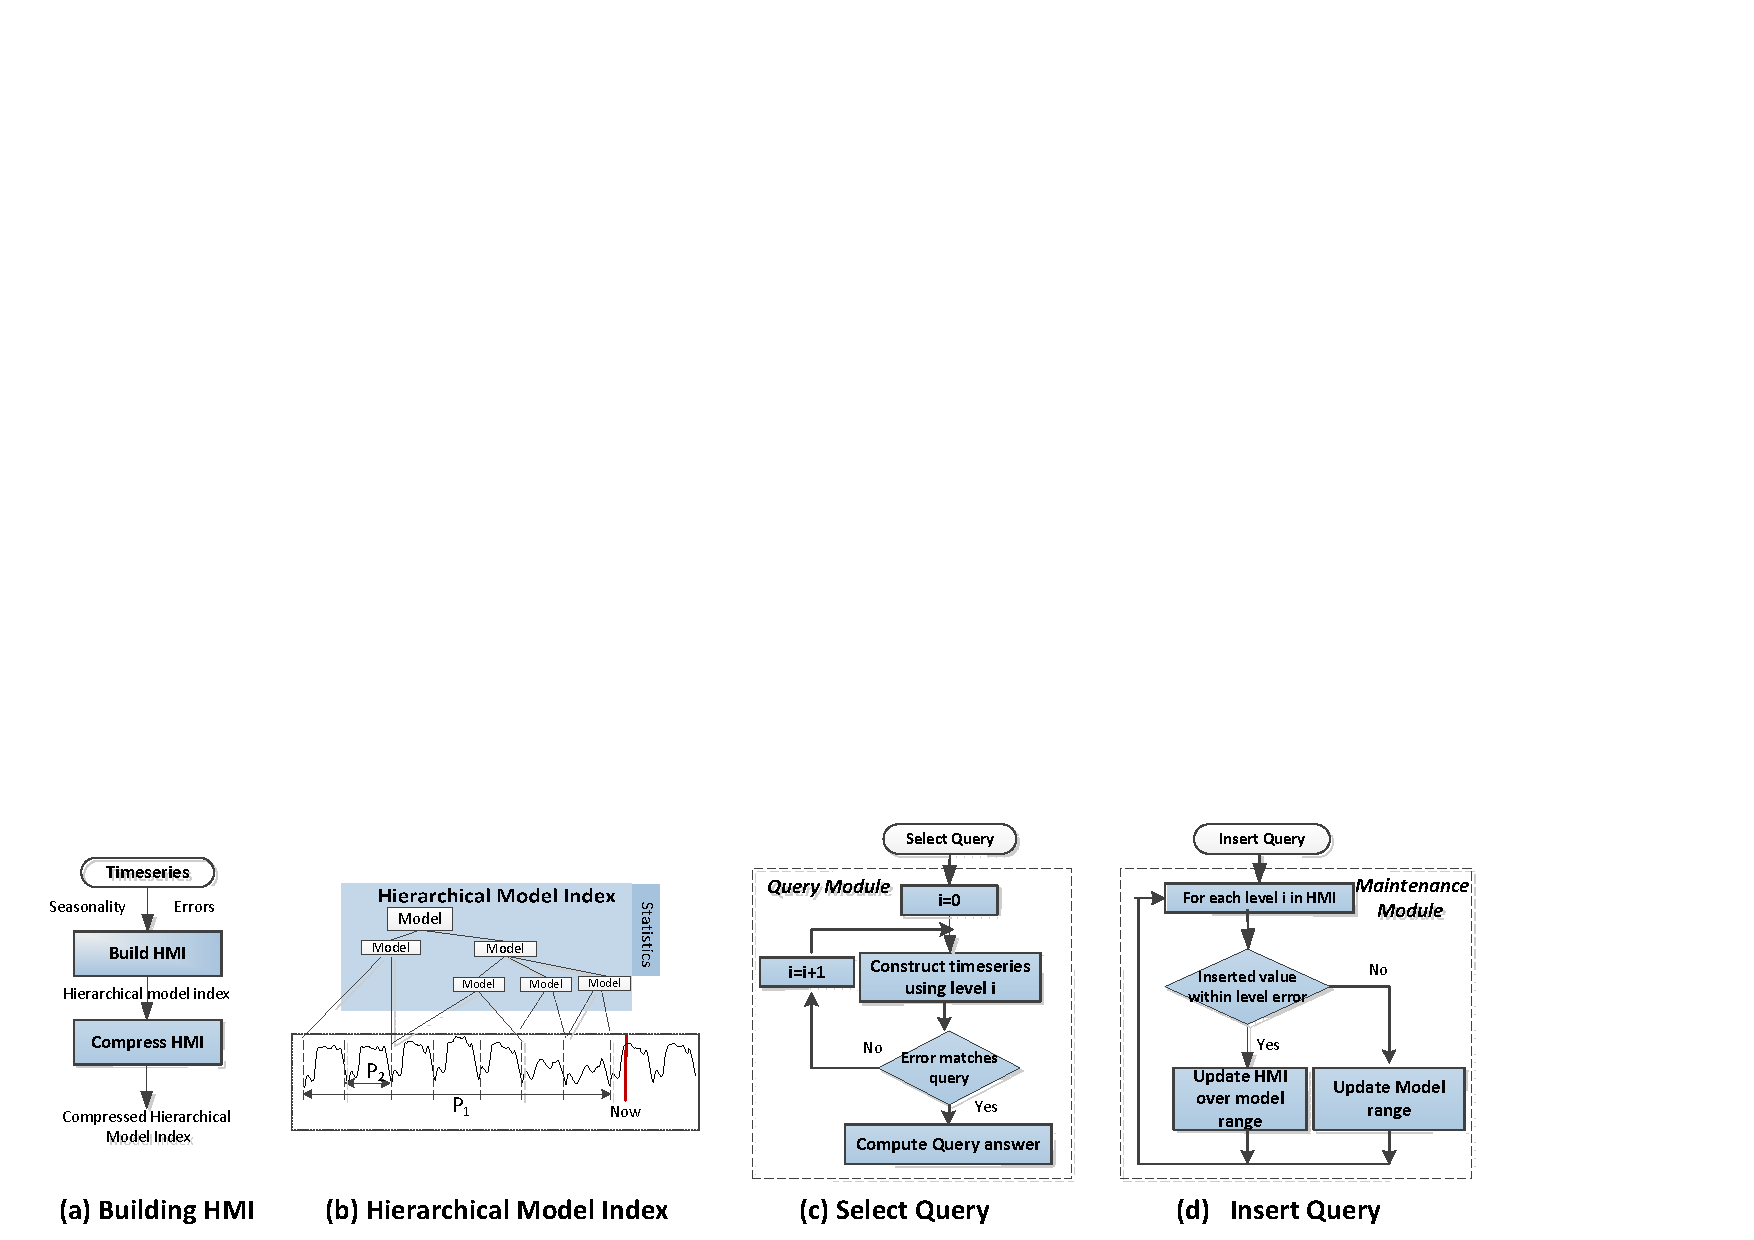
\includegraphics[width=6in]{figs/overview3.pdf}
%\caption{TimeTravel System Overview}
%\label{fig:arch}
%\end{figure*} 
\begin{figure}[th]
\center
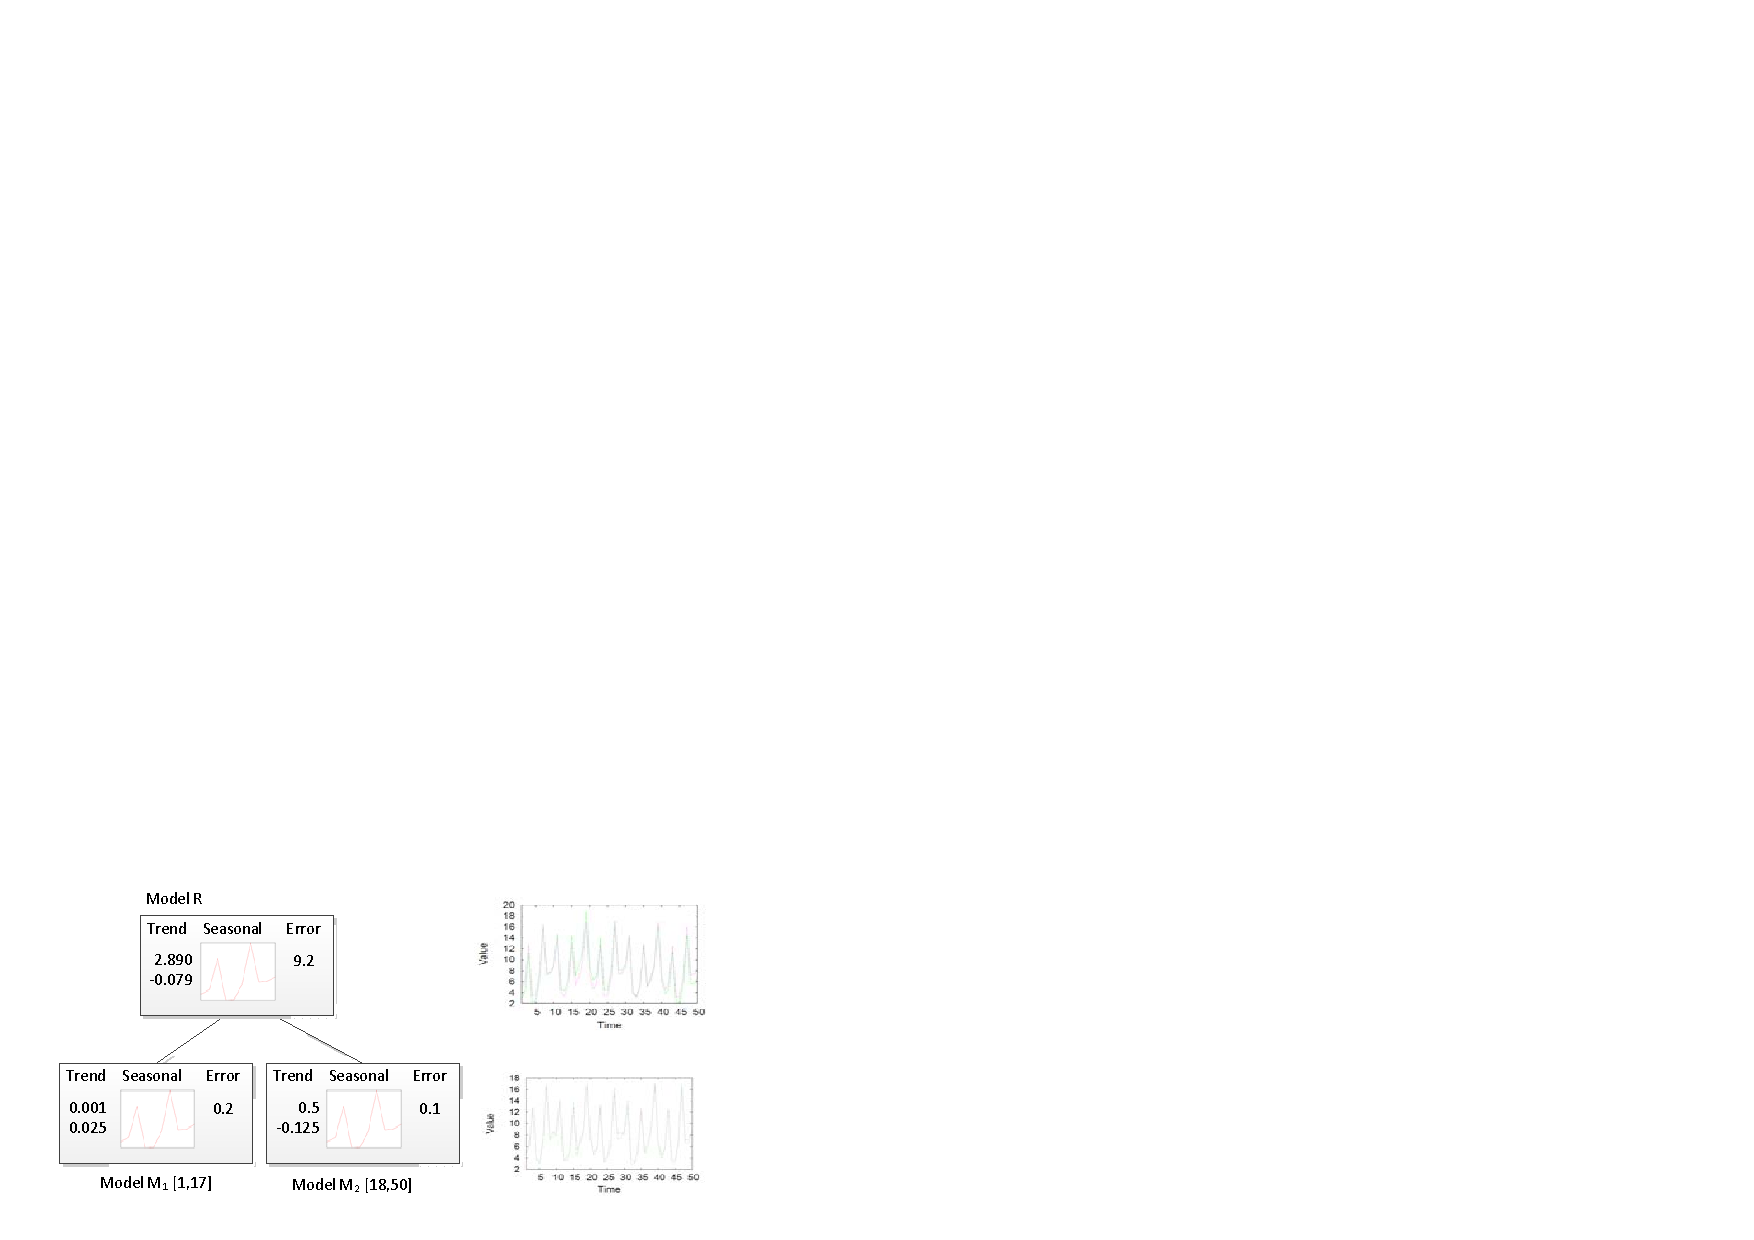
\includegraphics[width=3in]{figs/example_tree.pdf}
\caption{HMI for the motivating example}
\label{fig:exampletree}
\end{figure} 


